\section*{Instruction Manual}

\subsection*{Setting up the Hardware}

\begin{figure}[H]
	\begin{center}
		\begin{tikzpicture}
			\node[,inner sep=0] at (0,0) {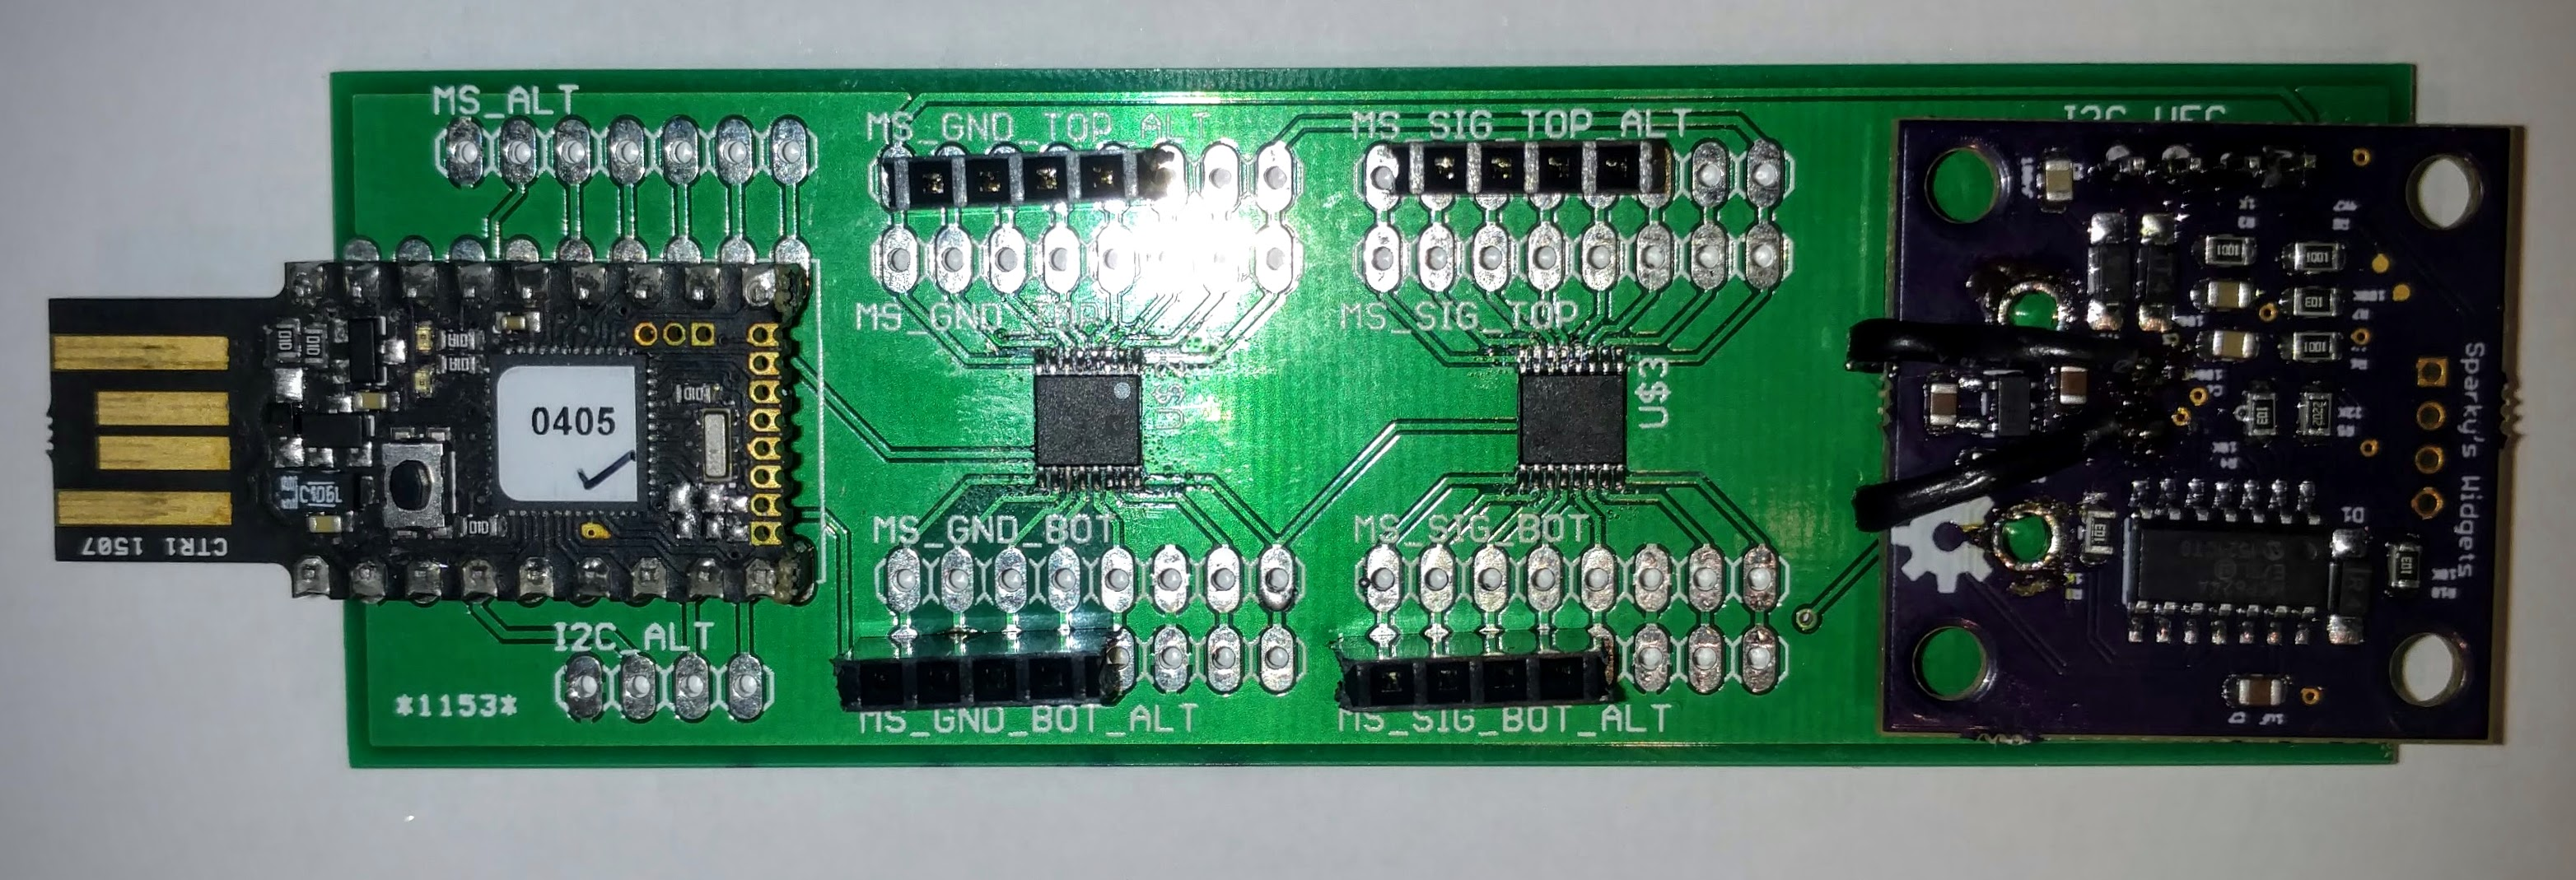
\includegraphics[width=0.5\textwidth]{images/cb.jpg}};
			\node[inner sep=0] at (0,-3) {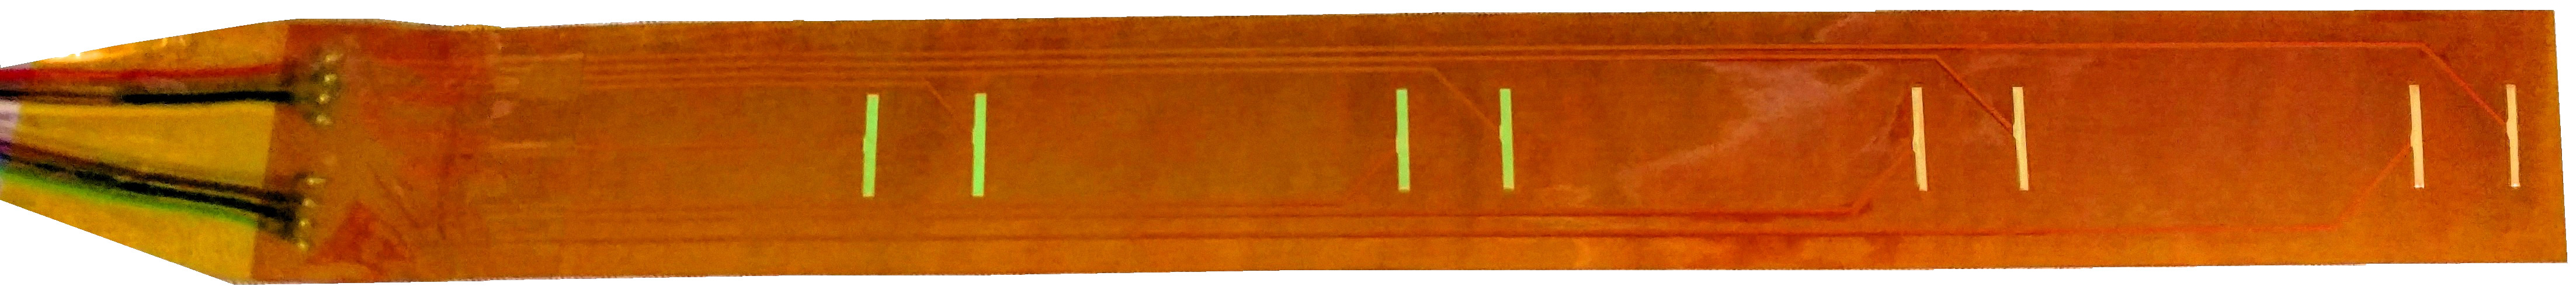
\includegraphics[width=\textwidth]{images/fpcbp.jpg}};
			
			\draw[red,ultra thick,rounded corners] (-4,-0.55) rectangle (-3.25,0.55);
			
			%\draw[red!50!yellow,ultra thick,rounded corners] (-1,-0.35) rectangle (-0.25,0.35);
			%\draw[red!50!yellow,ultra thick,rounded corners] (0.55,-0.35) rectangle (1.3,0.35);
			
			\draw[red!25!yellow,ultra thick,rounded corners] (-1.45,-1) rectangle (-0.3,-0.6);
			\draw[red!25!yellow,ultra thick,rounded corners] (0.3,-1.05) rectangle (1.3,-0.65);
			\draw[red!25!yellow,ultra thick,rounded corners] (-1.54,1.05) rectangle (-0.44,0.65);
			\draw[red!25!yellow,ultra thick,rounded corners] (0.15,1.05) rectangle (1.15,0.65);
			
			%\draw[blue,ultra thick,rounded corners] (1.8,-1.2) rectangle (4,1.2);
			\draw[blue!75!white,ultra thick,rounded corners] (-8,-4) rectangle (8,-2);
			%\draw[blue!50!white,ultra thick,rounded corners] (-2.75,-3.5) rectangle (-1.65,-2.5);
		\end{tikzpicture}
		\caption{USB connection (\drawline[red,ultra thick])\\sensor strip (\drawline[blue!75!white,ultra thick])\\connectors (\drawline[red!25!yellow,ultra thick])}
		\label{fig:isysa}
	\end{center}
\end{figure}

\begin{itemize}
	\item[1] Use electrical tape to mount the sensor strips at desired points of measurement. Make sure not to cover the electrodes (golden parts).
	\item[2] Connect the cables of the sensor strip to the carrier board as shown in the picture:
	\begin{figure}[H]
	\begin{center}
		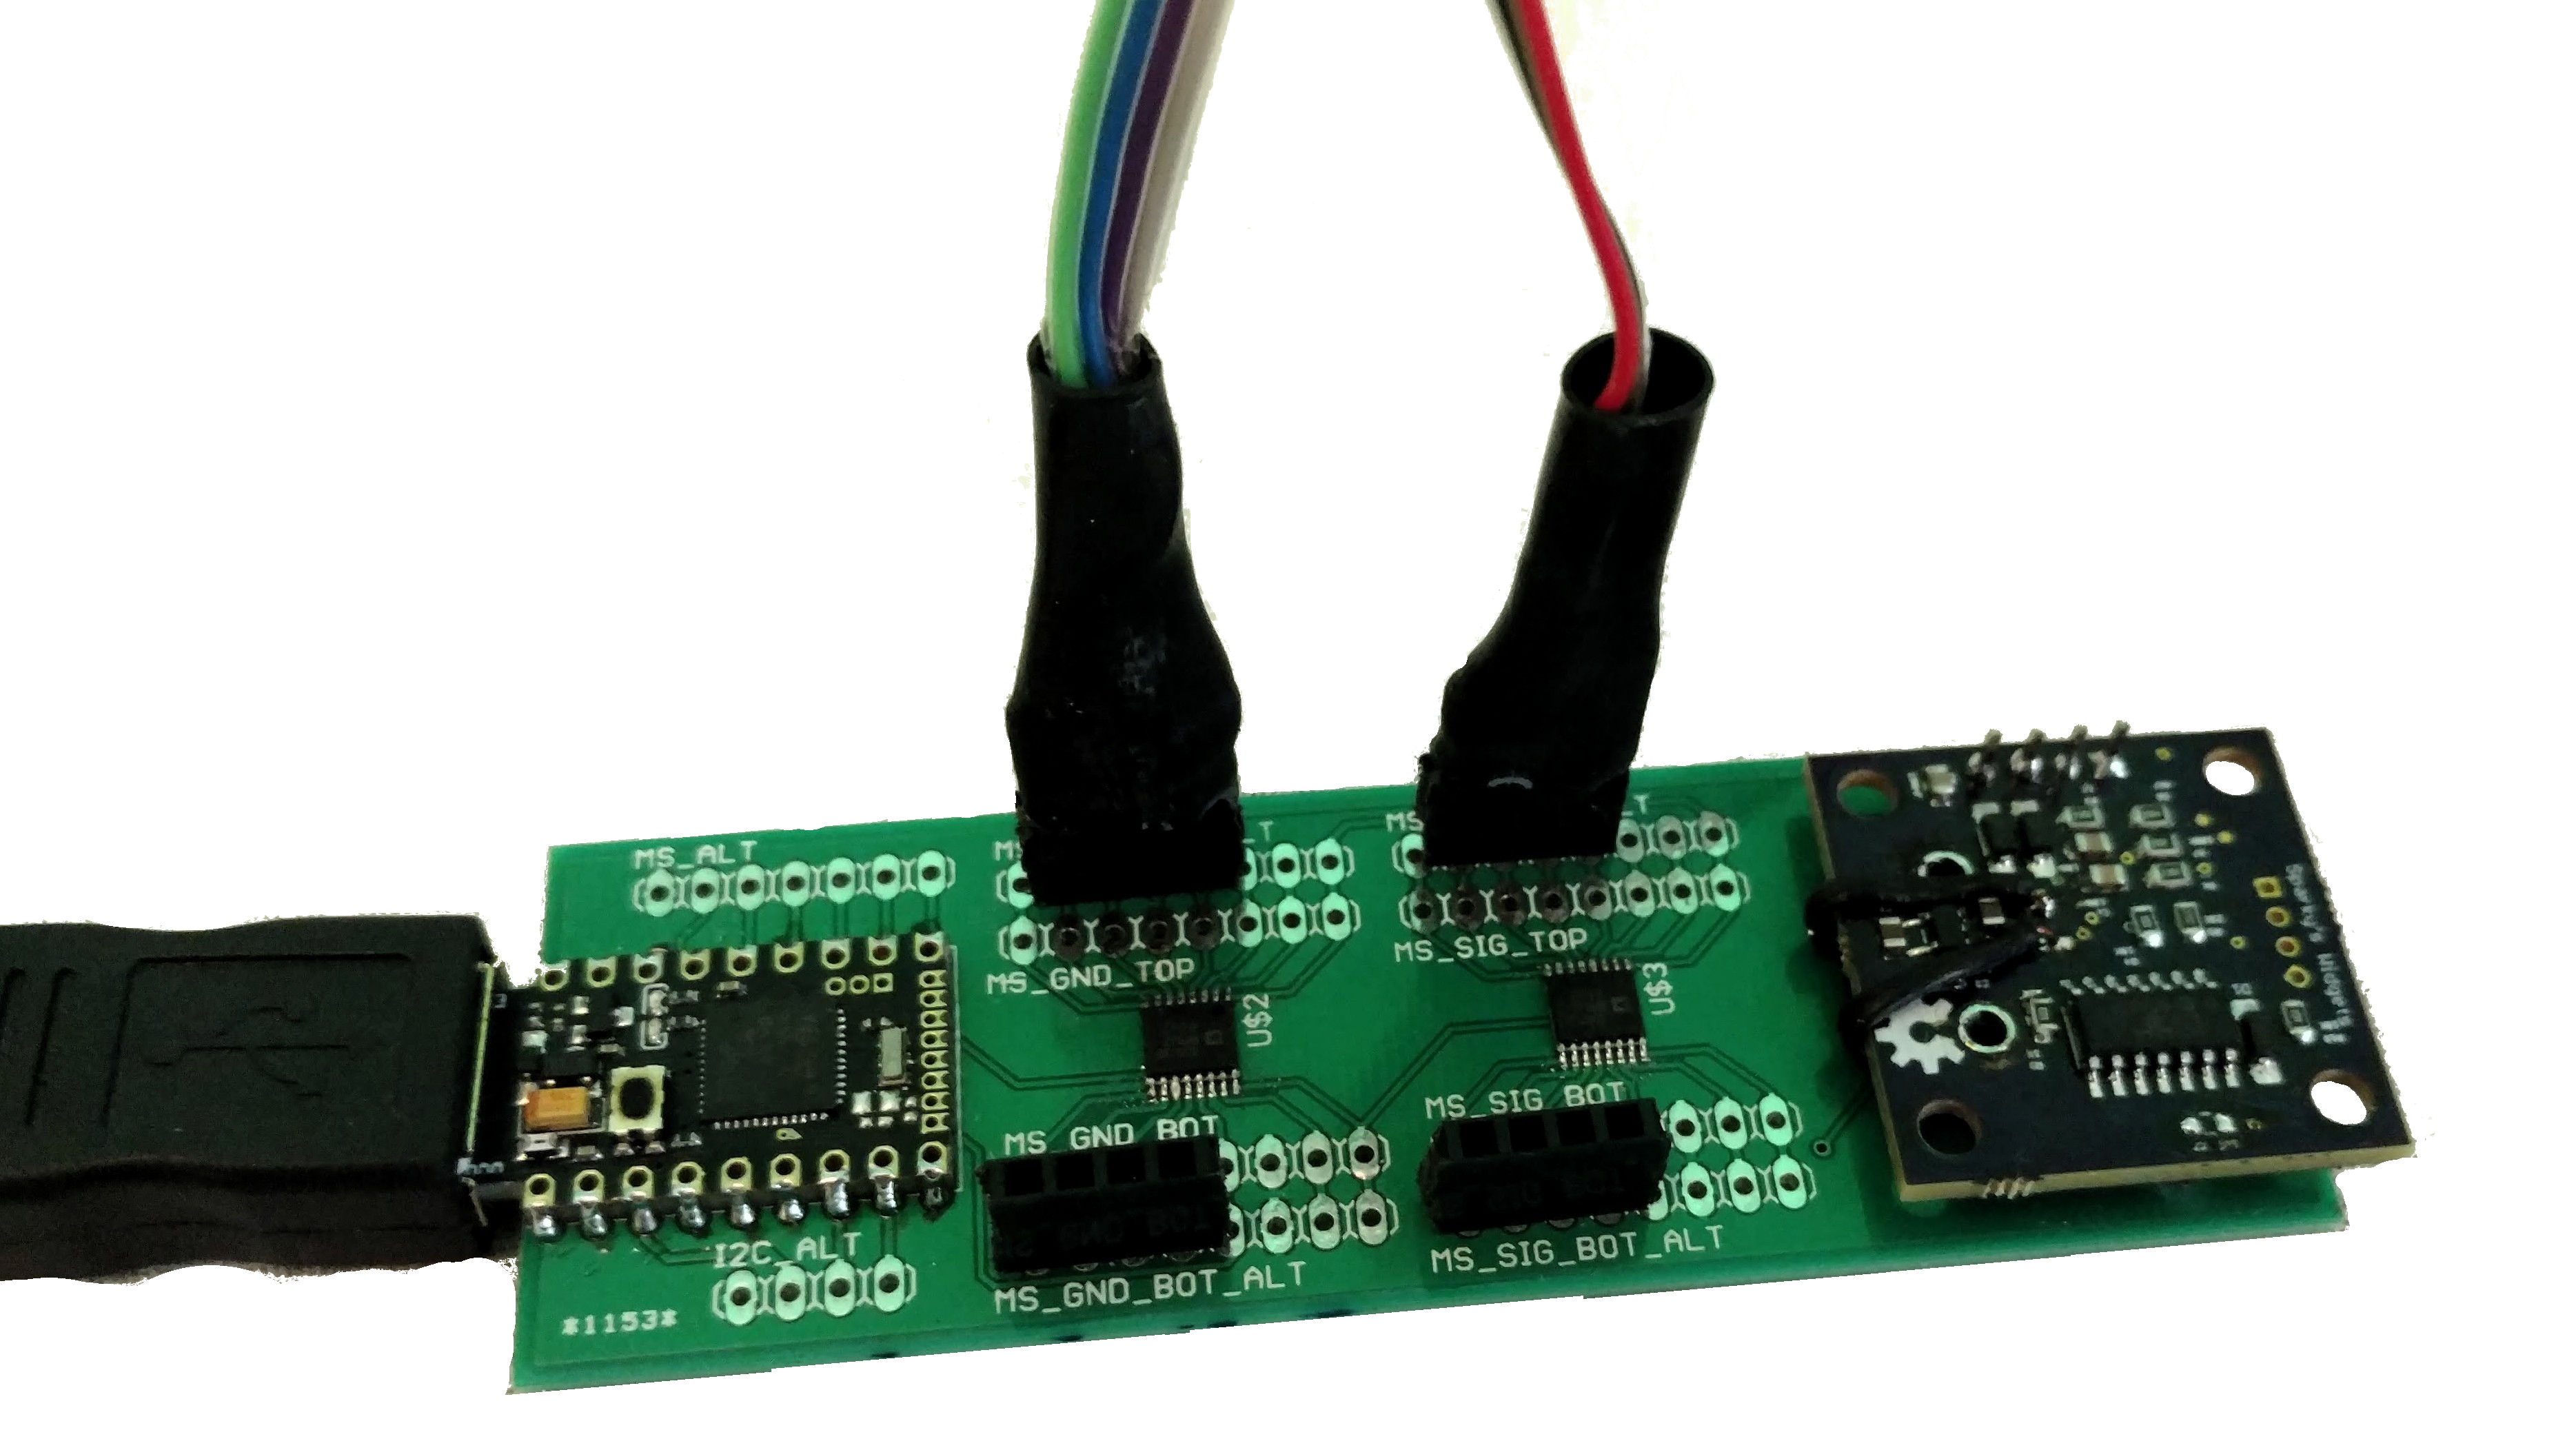
\includegraphics[width=0.5\textwidth]{images/conn.jpg}
		\caption{connectors}
		\label{fig:iconna}
	\end{center}
\end{figure}
	\item[3] Connect the carrier board to the host PC with the USB cable. Note the orientation in the picture:
		\begin{figure}[H]
	\begin{center}
		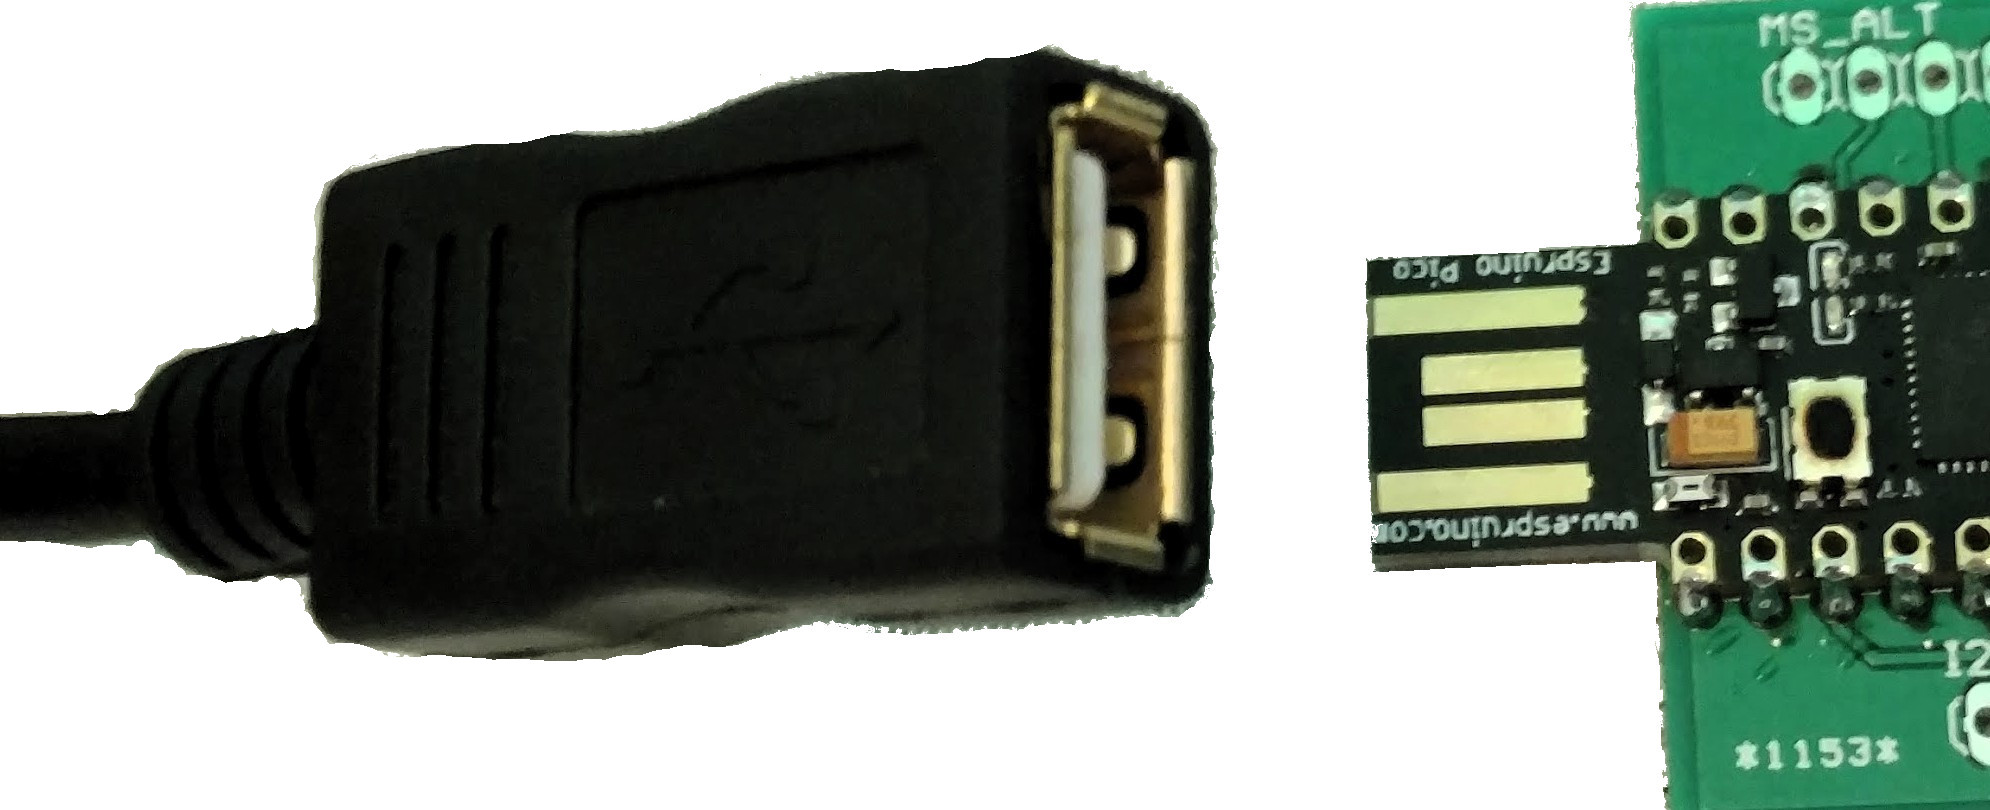
\includegraphics[width=0.5\textwidth]{images/usb.jpg}
		\caption{USB}
		\label{fig:iusba}
	\end{center}
\end{figure}
	Wrong orientation will not cause any damage, but the system will not work.
\end{itemize}

\subsection*{Capturing data using the OpenSalinityGUI}

\begin{itemize}
	\item[0] Follow the three steps of "Setting up the Hardware".
	\item[1] Start the OpenSalinity GUI by clicking on the icon.
	\item[2] Click "Save" on the top right to chose a file to log the data to. If you want to use the default filename, just click "Open" in the file menu.
	\item[3] Start the measurement by clicking "Start".
	\item[4] Stop the measurement by clicking "Stop".
	\item[5] Repeat from step 1 for all subsequent measurements. If no new file is chosen before starting a new measurement, the data is added at the end of the previous file.
\end{itemize}

\subsection*{Capturing data using command line tools}

\begin{itemize}
	\item[0] Follow the three steps of "Setting up the Hardware".
	\item[1] Open a terminal.
	\item[2] Change the working directory to the directory liveplot.sh is in:
	\begin{lstlisting}
		cd ~/path/to/directory
	\end{lstlisting}
	\item[3] Execute "liveplot.sh" with a file name as argument:
	\begin{lstlisting}
		./liveplot.sh log.csv
	\end{lstlisting}
	\item[4] To end data capturing, click into the terminal and press "Ctrl+C".
	\item[5] Repeat from step 1 for all subsequent measurements. If the file name is not changed, the existing file will be overwritten.
\end{itemize}